\section{\RU{Пример с сравнением}\EN{Comparison example}}

\RU{Попробуем теперь вот это:}\EN{Let's try this:}

\lstinputlisting{patterns/12_FPU/3_comparison/d_max.c}

\RU{Несмотря на кажущуюся простоту этой функции, понять, как она работает, будет чуть сложнее.}
\EN{Despite the simplicity of the function, it will be harder to understand how it works.}

% subsections
\subsection{x86}

% subsubsections
\subsubsection{\NonOptimizing MSVC}

\RU{Вот что выдал MSVC 2010}\EN{MSVC 2010 generated}:

\lstinputlisting[caption=\NonOptimizing MSVC 2010]{patterns/12_FPU/3_comparison/x86/MSVC/MSVC.asm.\LANG}

\index{x86!\Instructions!FLD}
\RU{Итак, \FLD загружает \TT{\_b} в регистр \ST{0}.}
\EN{So, \FLD loading \TT{\_b} into the \ST{0} register.}

\label{Czero_etc}
\newcommand{\Czero}{\TT{C0}\xspace}
\newcommand{\Ctwo}{\TT{C2}\xspace}
\newcommand{\Cthree}{\TT{C3}\xspace}
\newcommand{\CThreeBits}{\Cthree/\Ctwo/\Czero}

\index{x86!\Instructions!FCOMP}
\RU{\FCOMP сравнивает содержимое \ST{0} с тем что лежит в \TT{\_a} и выставляет биты \CThreeBits в 
регистре статуса FPU. Это 16-битный регистр отражающий текущее состояние FPU.}
\EN{\FCOMP compares the value in the \ST{0} register with what is in \TT{\_a} value 
and set \CThreeBits bits in FPU 
status word register. 
This is 16-bit register reflecting current state of FPU.}

\RU{После этого, инструкция \FCOMP также выдергивает одно значение из стека. 
Это отличает её от \FCOM, которая просто сравнивает значения, оставляя стек в таком же состоянии.}
\EN{After bits are set, the \FCOMP instruction also popping one variable from stack. 
This is what distinguish it from \FCOM, which is just comparing values, leaving the stack at the same state.}

\RU{К сожалению, у процессоров до Intel P6 
\footnote{Intel P6 это Pentium Pro, Pentium II, и далее} нет инструкций условного перехода,
проверяющих биты \CThreeBits. 
Возможно, так сложилось исторически (вспомните о том, что FPU когда-то был вообще отдельным чипом).\\
А у Intel P6 появились инструкции \FCOMI/\FCOMIP/\FUCOMI/\FUCOMIP ~--- делающие тоже самое, 
только напрямую модифицирующие флаги \ZF/\PF/\CF.}
\EN{Unfortunately, CPU before Intel P6
\footnote{Intel P6 is Pentium Pro, Pentium II, etc} has not any conditional 
jumps instructions, which are checking \CThreeBits bits. 
Probably, it is a matter of history (remember: FPU was separate chip in past).\\
Modern CPU starting at Intel P6 has \FCOMI/\FCOMIP/\FUCOMI/\FUCOMIP 
instructions~---which does the same, but modifies CPU flags \ZF/\PF/\CF.}

\index{x86!\Instructions!FNSTSW}
\RU{Так что \FNSTSW копирует содержимое регистра статуса в \AX. 
Биты \CThreeBits занимают позиции, 
соответственно, 14, 10, 8, в этих позициях они и остаются в регистре \AX, 
и все они расположены в старшей части регистра ~--- \AH.}
\EN{So the \FNSTSW instruction copies FPU status word register to the \AX. 
Bits \CThreeBits are placed at positions 14/10/8, 
they will be at the same positions in the \AX register and all they are placed in high part of the \AX{}~---\AH{}.}

\begin{itemize}
\item
\RU{Если $b>a$ в нашем случае, то биты \CThreeBits должны быть выставлены так:}
\EN{If $b>a$ in our example, then \CThreeBits bits will be set as following:} 0, 0, 0.
\item
\RU{Если $a>b$, то биты будут выставлены:}\EN{If $a>b$, then bits will be set:} 0, 0, 1.
\item
\RU{Если $a=b$, то биты будут выставлены так:}\EN{If $a=b$, then bits will be set:} 1, 0, 0.
\item
\RU{Если результат не определен (в случае ошибки), то биты будут выставлены так}\EN{If result 
is unordered (in case of error), then bits will be set}: 1, 1, 1.
\end{itemize}
% TODO: table here?

\EN{This is how \CThreeBits bits are located in the \AX register:}
\RU{Вот как биты \CThreeBits расположены в регистре \AX:}

\begin{center}
\begin{bytefield}[endianness=big,bitwidth=0.03\linewidth]{16}
\bitheader{14,10,9,8} \\
\bitbox{1}{} & 
\bitbox{1}{\TT{C3}} & 
\bitbox{3}{} & 
\bitbox{1}{\TT{C2}} & 
\bitbox{1}{\TT{C1}} & 
\bitbox{1}{\TT{C0}} &
\bitbox{8}{}
\end{bytefield}
\end{center}


\EN{This is how \CThreeBits bits are located in the \AH register:}
\RU{Вот как биты \CThreeBits расположены в регистре \AH:}

\begin{center}
\ifdefined\ebook
\begin{bytefield}[endianness=big,bitwidth=0.06\linewidth]{8}
\else
\begin{bytefield}[endianness=big,bitwidth=0.03\linewidth]{8}
\fi
\bitheader{6,2,1,0} \\
\bitbox{1}{} & 
\bitbox{1}{\TT{C3}} & 
\bitbox{3}{} & 
\bitbox{1}{\TT{C2}} & 
\bitbox{1}{\TT{C1}} & 
\bitbox{1}{\TT{C0}}
\end{bytefield}
\end{center}


\RU{После исполнения \TT{test ah, 5}\footnote{5=1001b}, % FIXME: subscript here!
будут учтены только биты \Czero и \Ctwo (на позициях 0 и 2), остальные проигнорированы.}
\EN{After \TT{test ah, 5} execution\footnote{5=1001b}, 
only \Czero and \Ctwo bits (on 0 and 2 position) will be considered, all other bits will be
ignored.}

\label{parity_flag}
\index{x86!\Registers!\Flags!\RU{Флаг четности}\EN{Parity flag}}
\RU{Теперь немного о \IT{parity flag}\footnote{флаг четности}. 
Еще один замечательный рудимент эпохи.}
\EN{Now let's talk about \IT{parity flag}. Another notable epoch rudiment.}

\RU{Этот флаг выставляется в $1$ если количество единиц в последнем результате ~--- четно. 
И в $0$ если ~--- нечетно.}
\EN{This flag is to be set to $1$ if number of ones in last calculation result is even. 
And to $0$ if odd.}

\RU{Заглянем в}\EN{Let's look into} Wikipedia
\footnote{\href{http://go.yurichev.com/17131}{wikipedia}}:

\begin{framed}
\begin{quotation}
One common reason to test the parity flag actually has nothing to do with parity. The FPU has four condition flags 
(C0 to C3), but they can not be tested directly, and must instead be first copied to the flags register. 
When this happens, C0 is placed in the carry flag, C2 in the parity flag and C3 in the zero flag. 
The C2 flag is set when e.g. incomparable floating point values (NaN or unsupported format) are compared 
with the FUCOM instructions.
\end{quotation}
\end{framed}

\EN{As noted in Wikipedia, the parity flag used sometimes in FPU code and let's see how.}
\RU{Как упоминается в Wikipedia, флаг четности иногда используется в FPU-коде и сейчас увидим, как.}

\index{x86!\Instructions!JP}
\RU{Флаг \PF будет выставлен в $1$, если \Czero и \Ctwo 
оба $1$ или оба $0$. 
И тогда сработает последующий \JP (\IT{jump if PF==1}). 
Если мы вернемся чуть назад и посмотрим значения \CThreeBits 
для разных вариантов, то увидим, что условный переход \JP сработает в двух случаях: если $b>a$ или если $a=b$ 
(ведь бит \Cthree перестал учитываться после исполнения \TT{test ah, 5}).}
\EN{The \PF flag will be set to 1 if both \Czero and \Ctwo are set to $0$ or both are $1$.
And then following \JP (\IT{jump if PF==1}) will be triggered. 
If we recall values of the \CThreeBits for various cases,
we will see the conditional jump 
\JP will be triggered in two cases: if $b>a$ or $a=b$ 
(\Cthree bit is not considering here since it was cleared while execution of 
the \TT{test ah, 5} instruction).}

\RU{Дальше все просто. Если условный переход сработал, то \FLD загрузит значение \TT{\_b} в \ST{0}, 
а если не сработал, то загрузится \TT{\_a} и произойдет выход из функции.}
\EN{It is all simple thereafter. If conditional jump was triggered, \FLD will load the \TT{\_b} value 
to the \ST{0} register, and if it is not triggered, the value of the \TT{\_a} variable will be loaded.}

\myparagraph{\RU{А как же проверка флага \Ctwo}\EN{What about \Ctwo flag checking}?}

\RU{Флаг \Ctwo включается в случае ошибки (\gls{NaN}, и т.д.), но наш код его не проверяет.}
\EN{\Ctwo flag is set in case of error (\gls{NaN}, etc), but our code doesn't check it.}
\RU{Если программисту нужно знать, не произошла ли FPU-ошибка, он должен позаботиться об этом
дополнительно, добавив соответствующие проверки.}
\EN{If programmer is aware about FPU errors, he/she must add additional checks.}

\ifdefined\IncludeOlly
\clearpage
\myparagraph{\RU{Первый пример с \olly}\EN{First \olly example}: a=1.2 \AndENRU b=3.4}
\index{\olly}

\RU{Загружаем пример в}\EN{Let's load the example into} \olly:

\begin{figure}[H]
\centering
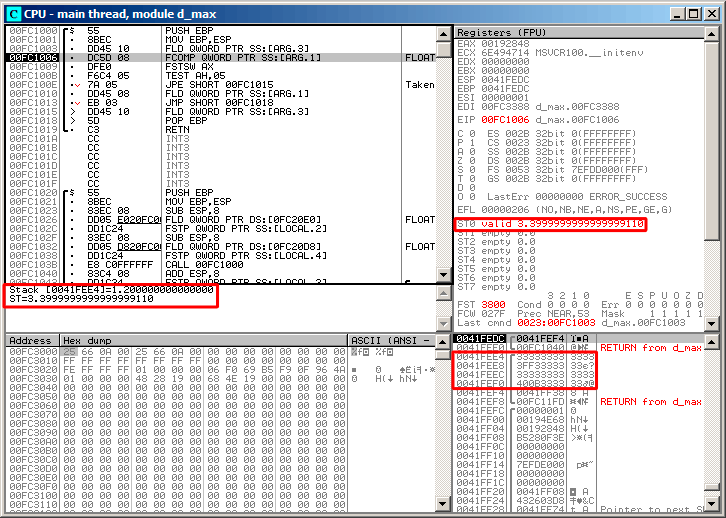
\includegraphics[scale=\FigScale]{patterns/12_FPU/3_comparison/x86/MSVC/olly1_1.png}
\caption{\olly: \RU{первая \FLD исполнилась}\EN{first \FLD is executed}}
\label{fig:FPU_comparison_case1_olly1}
\end{figure}

\RU{Текущие параметры ф-ции}\EN{Current arguments of the function}: $a=1.2$ \AndENRU $b=3.4$ 
(\RU{их видно в стеке: 2 пары 32-битных значений}\EN{We can see them in the stack: two pairs of 32-bit values}).
$b$ ($3.4$) \RU{уже загружено в}\EN{is already loaded in} \ST{0}.
\RU{Сейчас будет исполняться \FCOMP}\EN{Now \FCOMP will be executed}. 
\olly \RU{показывает второй аргумент для \FCOMP, который сейчас находится в стеке}\EN{shows the second \FCOMP
argument, which is in stack right now}.

\clearpage
\FCOMP \RU{отработал}\EN{is executed}:

\begin{figure}[H]
\centering
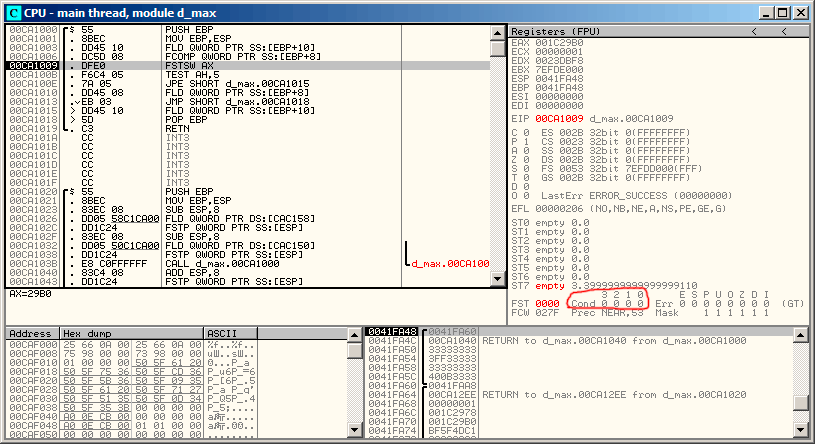
\includegraphics[scale=\FigScale]{patterns/12_FPU/3_comparison/x86/MSVC/olly1_2.png}
\caption{\olly: \FCOMP \RU{исполнилась}\EN{is executed}}
\label{fig:FPU_comparison_case1_olly2}
\end{figure}

\RU{Мы видим состояния condition-флагов \ac{FPU}}\EN{We see the state of the \ac{FPU}'s condition flags}: 
\RU{все нули}\EN{all zeroes}.
\RU{Вытолкнутое значение отображается как \ST{7}, почему это так, я писал раннее}
\EN{The popped value is reflected as \ST{7}, I wrote earlier about reason for this}: 
\ref{FPU_is_rather_circular_buffer}.

\clearpage
\FNSTSW \RU{сработал}\EN{is executed}:
\begin{figure}[H]
\centering
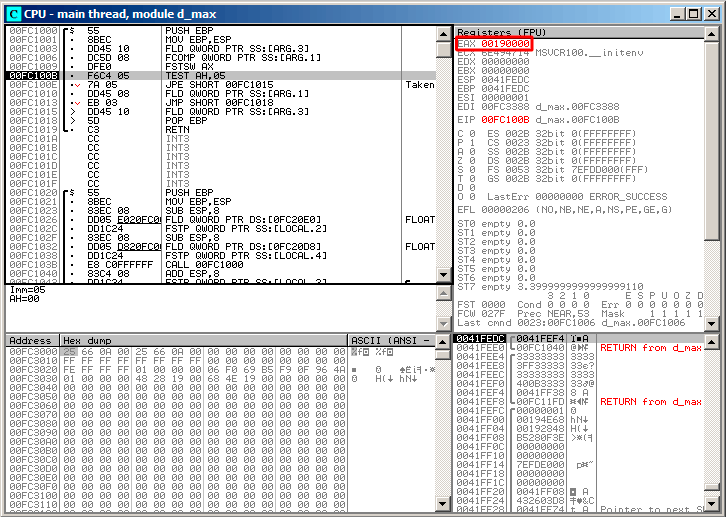
\includegraphics[scale=\FigScale]{patterns/12_FPU/3_comparison/x86/MSVC/olly1_3.png}
\caption{\olly: \FNSTSW \RU{исполнилась}\EN{is executed}}
\label{fig:FPU_comparison_case1_olly3}
\end{figure}

\RU{Видно, что регистр \TT{AX} содержит нули: действительно, ведь все condition-флаги тоже содержали нули.}
\EN{We see that the \TT{AX} register contain zeroes: indeed, all condition flags are zero.}
(\olly \RU{дизассемблирует команду}\EN{disassembles the} \FNSTSW \RU{как}\EN{instruction as} \TT{FSTSW} --- 
\RU{это синоним}\EN{they are synonyms}).

\clearpage
\TEST \RU{сработал}\EN{is executed}:

\begin{figure}[H]
\centering
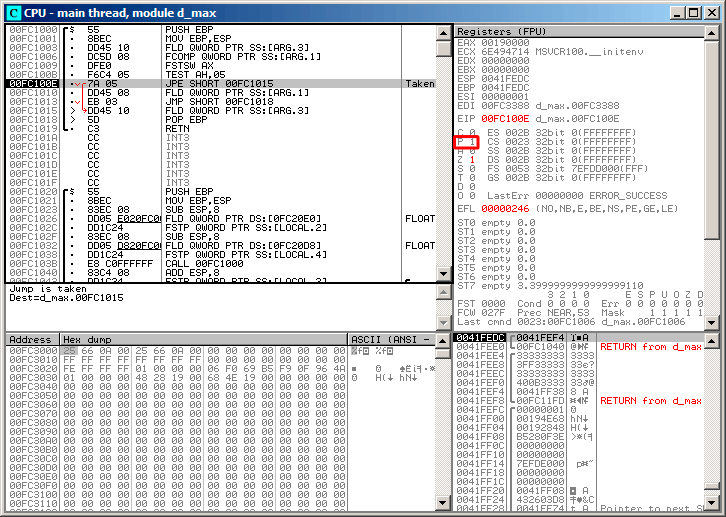
\includegraphics[scale=\FigScale]{patterns/12_FPU/3_comparison/x86/MSVC/olly1_4.png}
\caption{\olly: \TEST \RU{исполнилась}\EN{is executed}}
\label{fig:FPU_comparison_case1_olly4}
\end{figure}

\RU{Флаг \TT{PF} равен единице.}\EN{The \TT{PF} flag is set to $1$.}
\RU{Все верно: количество выставленных бит в $0$ --- это $0$, а $0$ --- это четное число.}
\EN{Indeed: the number of bits set in $0$ is $0$ and $0$ is an even number.}
\olly \RU{дизассемблирует}\EN{disassembles} \TT{JP} \RU{как}\EN{as} \ac{JPE} --- \RU{это синонимы}\EN{they
are synonyms}.
\RU{И она сейчас сработает}\EN{And it will trigger now}.

\clearpage
\ac{JPE} \RU{сработала}\EN{triggered}, \FLD \RU{загрузила в \ST{0} значение $b$ ($3.4$)}
\EN{loads the value of $b$ ($3.4$) in \ST{0}}:

\begin{figure}[H]
\centering
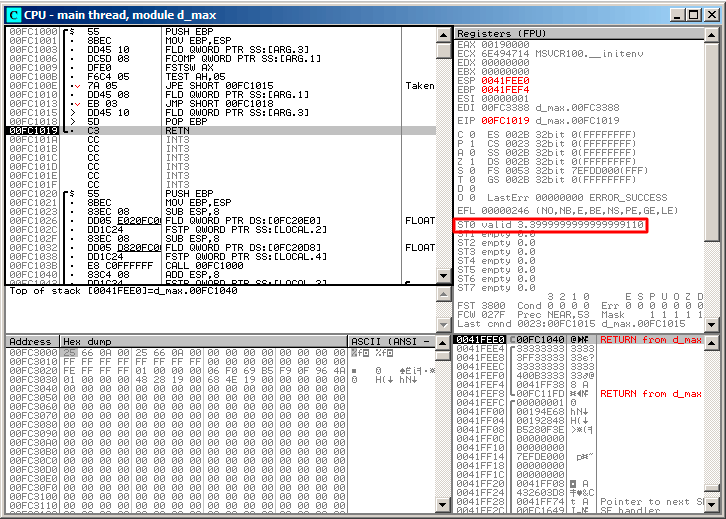
\includegraphics[scale=\FigScale]{patterns/12_FPU/3_comparison/x86/MSVC/olly1_5.png}
\caption{\olly: \RU{вторая \FLD исполнилась}\EN{second \FLD is executed}}
\label{fig:FPU_comparison_case1_olly5}
\end{figure}

\RU{Ф-ция заканчивает свою работу}\EN{The function finishes its work}.

\clearpage
\myparagraph{\RU{Второй пример с \olly}\EN{Second \olly example}: a=5.6 \AndENRU b=-4}

\RU{Загружаем пример в}\EN{Let's load example into} \olly:

\begin{figure}[H]
\centering
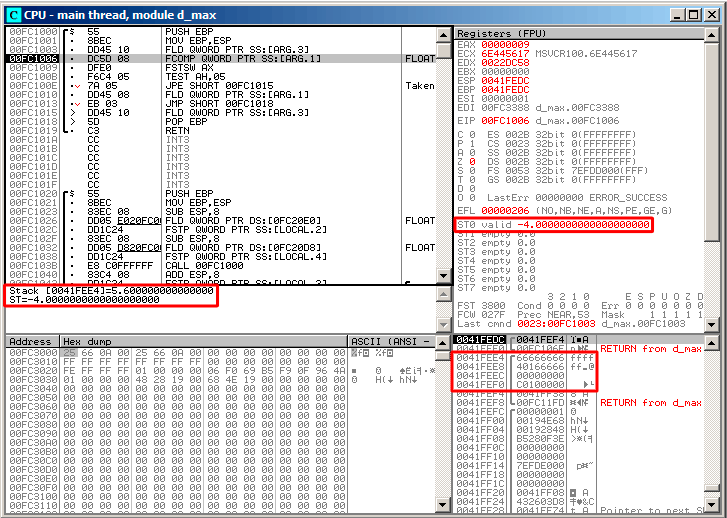
\includegraphics[scale=\FigScale]{patterns/12_FPU/3_comparison/x86/MSVC/olly2_1.png}
\caption{\olly: \RU{первая \FLD исполнилась}\EN{first \FLD executed}}
\label{fig:FPU_comparison_case2_olly1}
\end{figure}

\RU{Текущие параметры ф-ции}\EN{Current function arguments}: $a=5.6$ \AndENRU $b=-4$).
$b$ ($-4$) \RU{уже загружено в}\EN{is already loaded in} \ST{0}.
\RU{Сейчас будет исполняться \FCOMP}\EN{\FCOMP will execute now}. 
\olly \RU{показывает второй аргумент \FCOMP, который сейчас находится в стеке}
\EN{shows the second \FCOMP argument, which is in stack right now}.

\clearpage
\FCOMP \RU{отработал}\EN{executed}:

\begin{figure}[H]
\centering
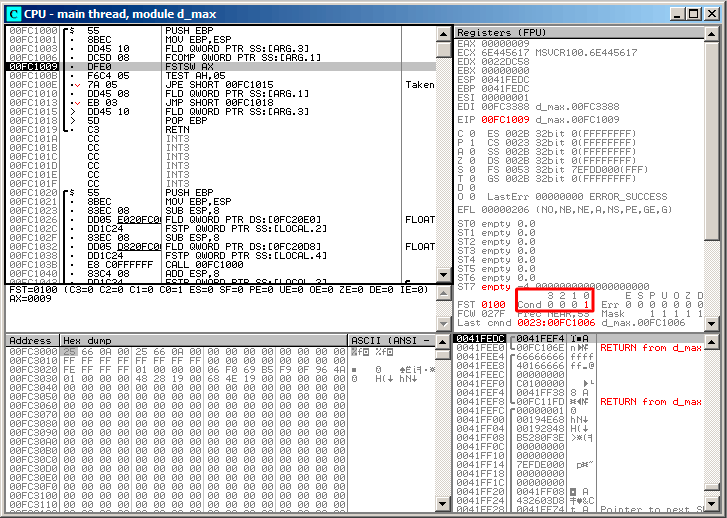
\includegraphics[scale=\FigScale]{patterns/12_FPU/3_comparison/x86/MSVC/olly2_2.png}
\caption{\olly: \FCOMP \RU{исполнилась}\EN{executed}}
\label{fig:FPU_comparison_case2_olly2}
\end{figure}

\RU{Мы видим значения condition-флагов \ac{FPU}: все нули кроме \Czero.}
\EN{We see the state of the \ac{FPU}'s condition flags: all zeroes except \Czero.}

\clearpage
\FNSTSW \RU{сработал}\EN{executed}:

\begin{figure}[H]
\centering
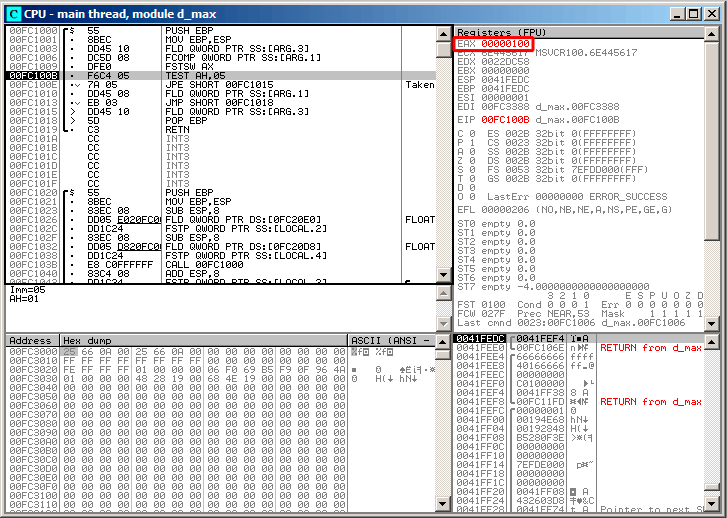
\includegraphics[scale=\FigScale]{patterns/12_FPU/3_comparison/x86/MSVC/olly2_3.png}
\caption{\olly: \FNSTSW \RU{исполнилась}\EN{executed}}
\label{fig:FPU_comparison_case2_olly3}
\end{figure}

\RU{Видно, что регистр \TT{AX} содержит \TT{0x100}: флаг \Czero стал на место 16-го бита.}
\EN{We see that the \TT{AX} register contains \TT{0x100}: the \Czero flag is at the 16th bit.}

\clearpage
\TEST \RU{сработал}\EN{executed}:

\begin{figure}[H]
\centering
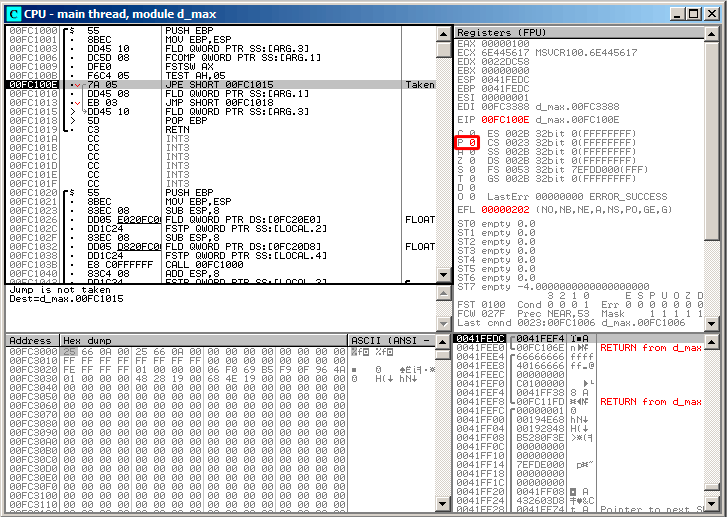
\includegraphics[scale=\FigScale]{patterns/12_FPU/3_comparison/x86/MSVC/olly2_4.png}
\caption{\olly: \TEST \RU{исполнилась}\EN{executed}}
\label{fig:FPU_comparison_case2_olly4}
\end{figure}

\EN{The}\RU{Флаг} \TT{PF} \RU{равен нулю}\EN{ flag is cleared}.
\RU{Все верно}\EN{Indeed}: 
\RU{количество единичных бит в \TT{0x100} --- это $1$, а $1$ --- это нечетное число}
\EN{the count of bits set in \TT{0x100} is $1$ and $1$ is an odd number}.
\ac{JPE} \RU{сейчас не сработает}\EN{will not be triggered}.

\clearpage
\ac{JPE} \RU{не сработала, }\EN{wasn't triggered, so} \FLD 
\RU{загрузила в \ST{0} значение $a$ ($5.6$)}
\EN{loads the value of $a$ ($5.6$) in \ST{0}}:

\begin{figure}[H]
\centering
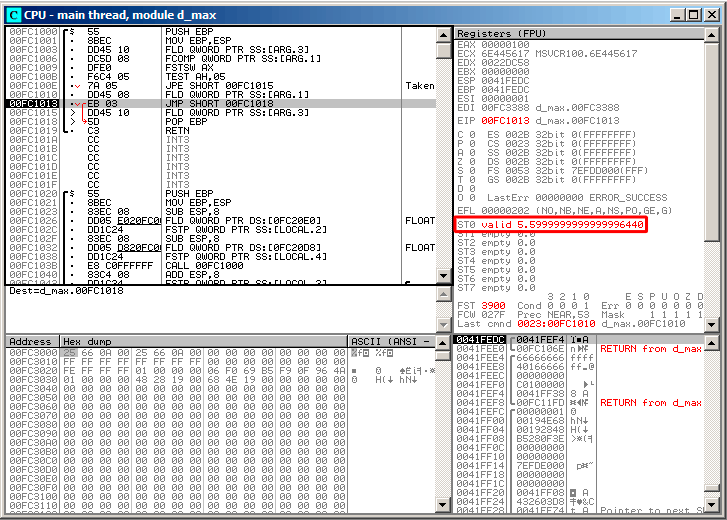
\includegraphics[scale=\FigScale]{patterns/12_FPU/3_comparison/x86/MSVC/olly2_5.png}
\caption{\olly: \RU{вторая \FLD исполнилась}\EN{second \FLD executed}}
\label{fig:FPU_comparison_case2_olly5}
\end{figure}

\RU{Ф-ция заканчивает свою работу}\EN{The function finishes its work}.

\fi

\subsubsection{\Optimizing MSVC 2010}

\lstinputlisting[caption=\Optimizing MSVC 2010]{patterns/12_FPU/3_comparison/x86/MSVC_Ox/\LANG.asm}

\index{x86!\Instructions!FCOM}
\RU{\FCOM отличается от \FCOMP тем что просто сравнивает значения и оставляет стек в том же состоянии. 
В отличие от предыдущего примера, операнды здесь в другом порядке. 
Поэтому и результат сравнения в \CThreeBits будет другим чем раньше:}
\EN{\FCOM is distinguished from \FCOMP in that sense that it just comparing values and leaves FPU stack 
in the same state. 
Unlike previous example, operands here in reversed order. 
And that is why result of comparison in the \CThreeBits will be different:}

\begin{itemize}
\item
\RU{Если a>b в нашем случае, то биты \CThreeBits должны быть выставлены так:}
\EN{If a>b in our example, then \CThreeBits bits will be set as:} 0, 0, 0.
\item
\RU{Если b>a, то биты будут выставлены:}\EN{If b>a, then bits will be set as:} 0, 0, 1.
\item
\RU{Если a=b, то биты будут выставлены так:}\EN{If a=b, then bits will be set as:} 1, 0, 0.
\end{itemize}
% TODO: table?

\RU{Инструкция \TT{test ah, 65} как бы оставляет только два бита ~--- \Cthree и \Czero. 
Они оба будут нулями, если a>b: в таком случае переход \JNE не сработает. 
Далее имеется инструкция \TT{FSTP ST(1)} ~--- эта инструкция копирует 
значение \ST{0} в указанный операнд и выдергивает одно значение из стека. В данном случае, 
она копирует \ST{0} 
(где сейчас лежит \TT{\_a}) в \ST{1}. 
После этого на вершине стека два раза лежат \TT{\_a}. Затем одно значение выдергивается. 
После этого в \ST{0} остается \TT{\_a} и функция завершается.}
\EN{It can be said, \TT{test ah, 65} instruction just leaves two bits~---\Cthree and \Czero. 
Both will be zeroes if \TT{a>b}: in that case \JNE jump will not be triggered. 
Then \TT{FSTP ST(1)} is following~---this instruction copies value in the \ST{0} into operand and 
popping one value from FPU stack.
In other words, the instruction copies \ST{0} (where \TT{\_a} value is now) into the \ST{1}.
After that, two values of the {\_a} are at the top of stack now. 
After that, one value is popping.
After that, \ST{0} will contain {\_a} and function is finished.}

\RU{Условный переход \JNE сработает в двух других случаях: если b>a или a==b. 
\ST{0} скопируется в \ST{0}, что как бы холостая операция, 
затем одно значение из стека вылетит и на вершине стека останется то что 
до этого лежало в \ST{1} (то есть, \TT{\_b}). И функция завершится. 
Эта инструкция используется здесь видимо потому что в FPU нет инструкции которая просто выдергивает 
значение из стека и выбрасывает его.}
\EN{Conditional jump \JNE is triggered in two cases: of b>a or a==b. 
\ST{0} into \ST{0} will be copied, it is just like idle (\ac{NOP}) operation, then one value 
is popping from stack and top of stack (\ST{0}) will contain what was in the \ST{1} before 
(that is {\_b}). Then function finishes. 
The instruction used here probably since \ac{FPU} has no instruction to pop value from stack and 
discard it.}

\myparagraph{\RU{Первый пример с \olly}\EN{First \olly example}: a=1.2 \AndENRU b=3.4}

\RU{Обе}\EN{Both} \FLD \RU{отработали}\EN{executed}: \figref{fig:FPU_comparison_Ox_case1_olly1}.
\RU{Сейчас будет исполняться }\FCOMP\EN{ being executed}: 
\olly \RU{показывает содержимое}\EN{shows contents of} \ST{0} \AndENRU \ST{1}, \RU{для удобства}
\EN{for convenience}.

\FCOM \RU{сработала}\EN{is done}: \figref{fig:FPU_comparison_Ox_case1_olly2}.
\Czero \RU{установлен, остальные флаги сброшены}\EN{is set, all other condition flags are cleared}.

\FNSTSW \RU{сработала}\EN{is done}, \TT{AX}=0x3100: \figref{fig:FPU_comparison_Ox_case1_olly3}.

\TEST \RU{сработала}\EN{executed}: \figref{fig:FPU_comparison_Ox_case1_olly4}.
ZF=0, \RU{переход сейчас произойдет}\EN{conditional jump will trigger now}.

\TT{FSTP ST} (\OrENRU \FSTP \ST{0}) \RU{сработала}\EN{executed}: $1.2$ 
\RU{было вытолкнуто из стека, и на вершине осталось $3.4$}\EN{was popped from the stack,
and $3.4$ was left on top of it}.
\figref{fig:FPU_comparison_Ox_case1_olly5}.
\RU{Видно, что инструкция}\EN{We see that the} \TT{FSTP ST} 
\RU{работает просто как выталкивание одного значения из FPU-стека}
\EN{instruction works just like popping one value from FPU-stack}.

\begin{figure}[H]
\centering
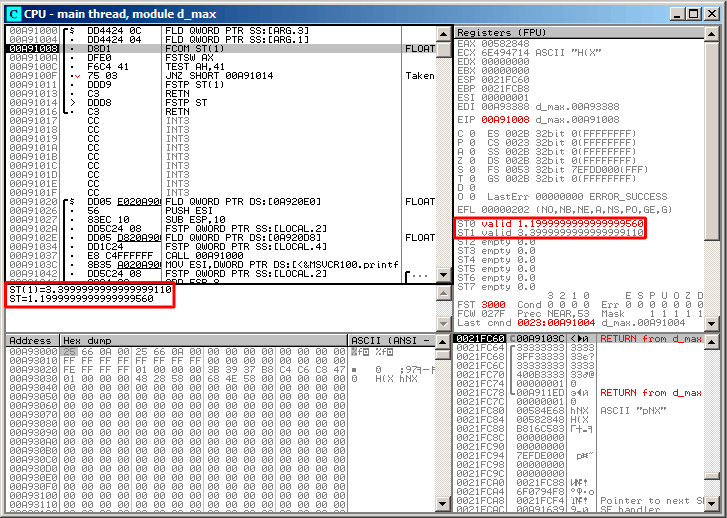
\includegraphics[scale=\FigScale]{patterns/12_FPU/3_comparison/x86/MSVC_Ox/olly1_1.png}
\caption{\olly: \RU{обе \FLD исполнились}\EN{both \FLD executed}}
\label{fig:FPU_comparison_Ox_case1_olly1}
\end{figure}

\begin{figure}[H]
\centering
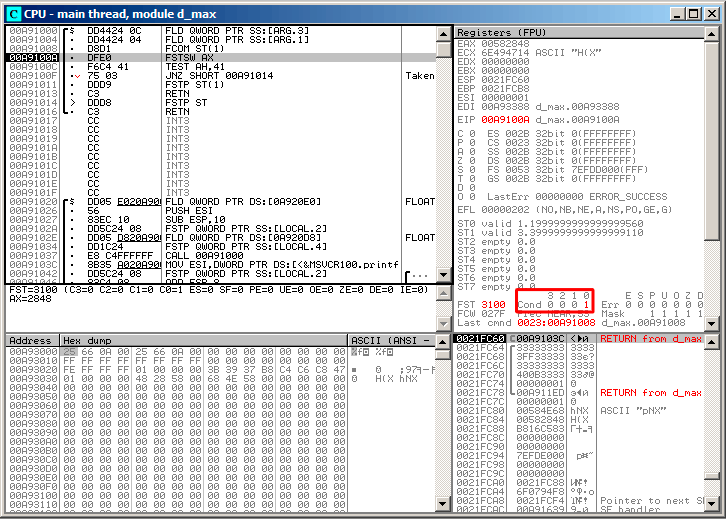
\includegraphics[scale=\FigScale]{patterns/12_FPU/3_comparison/x86/MSVC_Ox/olly1_2.png}
\caption{\olly: \FCOM \RU{исполнилась}\EN{executed}}
\label{fig:FPU_comparison_Ox_case1_olly2}
\end{figure}

\begin{figure}[H]
\centering
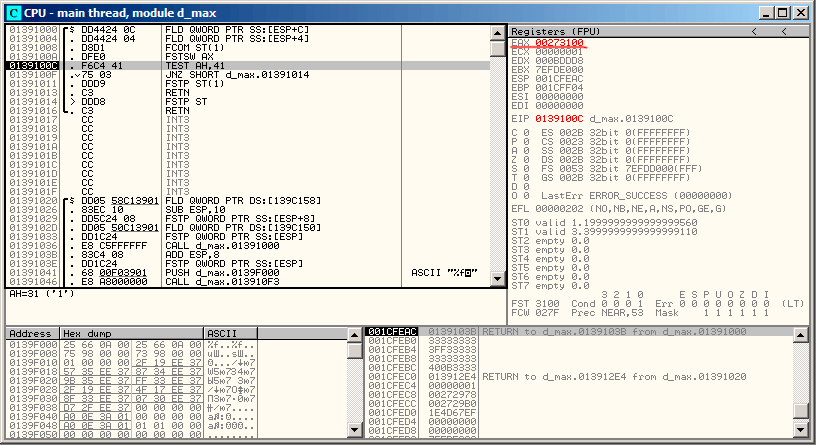
\includegraphics[scale=\FigScale]{patterns/12_FPU/3_comparison/x86/MSVC_Ox/olly1_3.png}
\caption{\olly: \FNSTSW \RU{исполнилась}\EN{executed}}
\label{fig:FPU_comparison_Ox_case1_olly3}
\end{figure}

\begin{figure}[H]
\centering
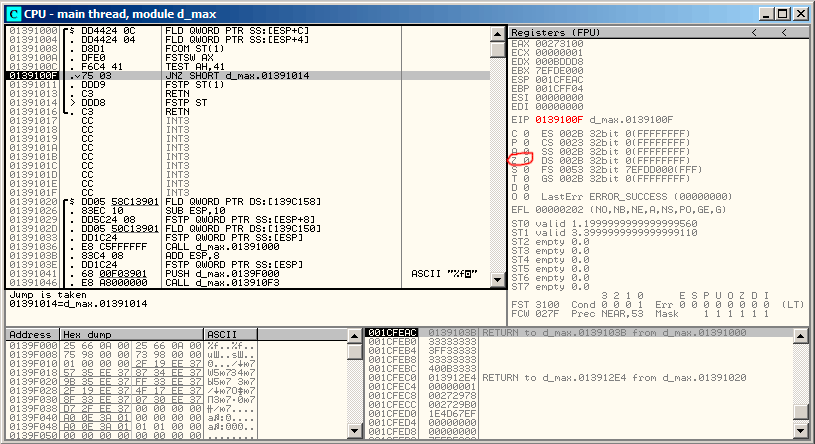
\includegraphics[scale=\FigScale]{patterns/12_FPU/3_comparison/x86/MSVC_Ox/olly1_4.png}
\caption{\olly: \TEST \RU{исполнилась}\EN{executed}}
\label{fig:FPU_comparison_Ox_case1_olly4}
\end{figure}

\begin{figure}[H]
\centering
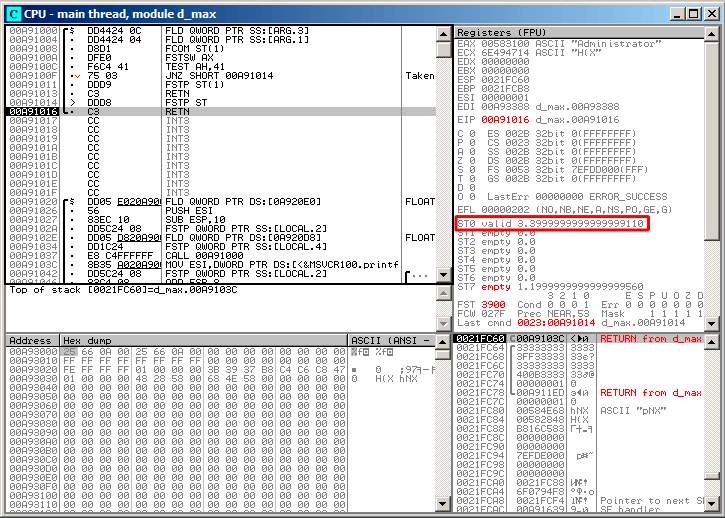
\includegraphics[scale=\FigScale]{patterns/12_FPU/3_comparison/x86/MSVC_Ox/olly1_5.png}
\caption{\olly: \FSTP \RU{исполнилась}\EN{executed}}
\label{fig:FPU_comparison_Ox_case1_olly5}
\end{figure}

\myparagraph{\RU{Второй пример с \olly}\EN{Second \olly example}: a=5.6 \AndENRU b=-4}

\RU{Обе}\EN{Both} \FLD \RU{отработали}\EN{executed}: \figref{fig:FPU_comparison_Ox_case2_olly1}.
\RU{Сейчас будет исполняться }\FCOMP\EN{ being executed}.

\FCOM \RU{сработала}\EN{done}: \figref{fig:FPU_comparison_Ox_case2_olly2}.
\RU{Все condition-флаги сброшены}\EN{All condition-flags are cleared}.

\FNSTSW \RU{сработала}\EN{done}, \TT{AX}=0x3000: \figref{fig:FPU_comparison_Ox_case2_olly3}.

\TEST \RU{сработала}\EN{is done}: \figref{fig:FPU_comparison_Ox_case2_olly4}.
ZF=1, \RU{переход сейчас не произойдет}\EN{jump will not be triggered now}.

\FSTP \ST{1} \RU{сработала: на вершине FPU-стека осталось значение $5.6$}\EN{was executed: a value
of $5.6$ is now at the top of FPU-stack}.
\figref{fig:FPU_comparison_Ox_case2_olly5}.
\RU{Видно, что инструкция}\EN{We now see that} \FSTP \ST{1} 
\RU{работает так: оставляет значение на вершине стека, но обнуляет регистр \ST{1}}
\EN{instruction works as follows: it leaves what was at the top of stack, but clears \ST{1} register}.

\begin{figure}[H]
\centering
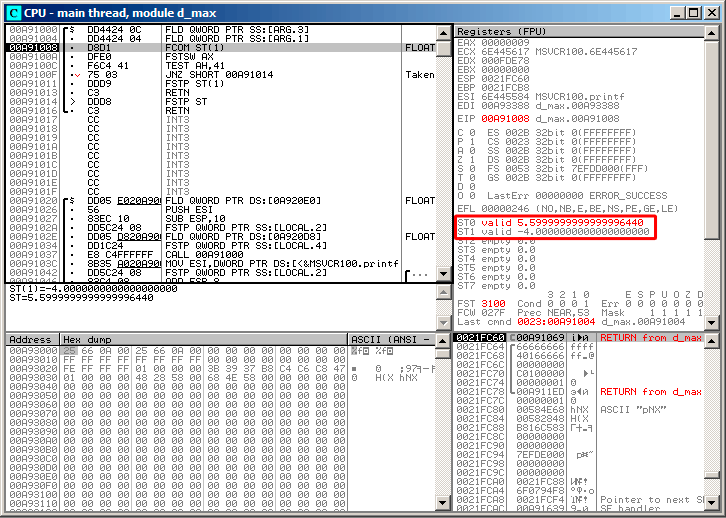
\includegraphics[scale=\FigScale]{patterns/12_FPU/3_comparison/x86/MSVC_Ox/olly2_1.png}
\caption{\olly: \RU{обе \FLD исполнились}\EN{both \FLD executed}}
\label{fig:FPU_comparison_Ox_case2_olly1}
\end{figure}

\begin{figure}[H]
\centering
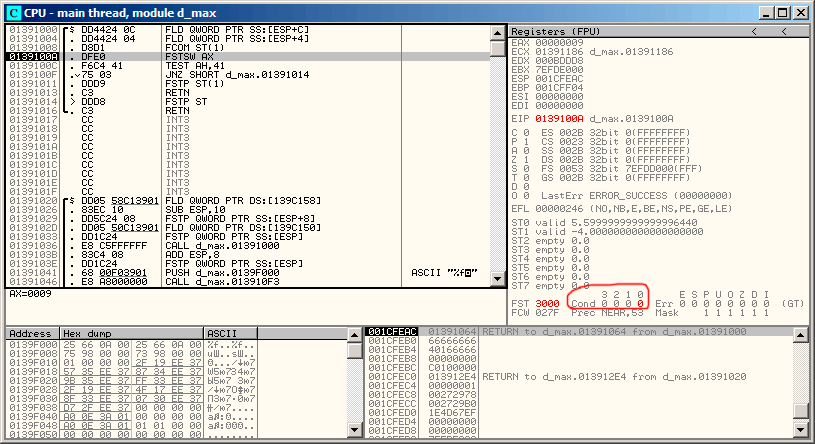
\includegraphics[scale=\FigScale]{patterns/12_FPU/3_comparison/x86/MSVC_Ox/olly2_2.png}
\caption{\olly: \FCOM \RU{исполнилась}\EN{executed}}
\label{fig:FPU_comparison_Ox_case2_olly2}
\end{figure}

\begin{figure}[H]
\centering
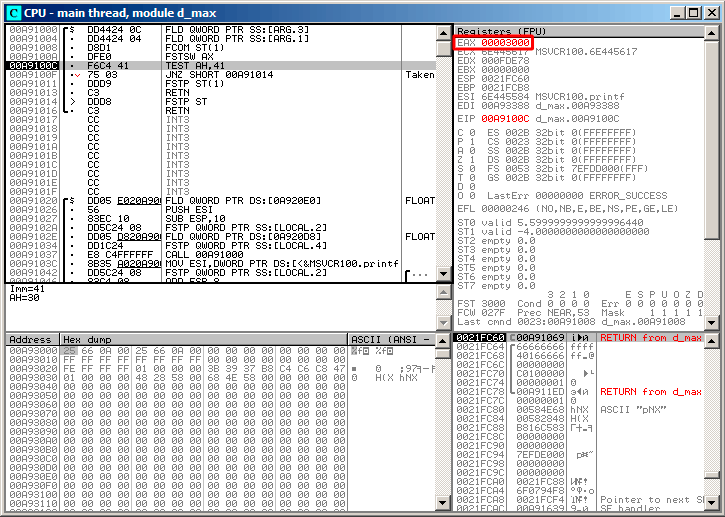
\includegraphics[scale=\FigScale]{patterns/12_FPU/3_comparison/x86/MSVC_Ox/olly2_3.png}
\caption{\olly: \FNSTSW \RU{исполнилась}\EN{executed}}
\label{fig:FPU_comparison_Ox_case2_olly3}
\end{figure}

\begin{figure}[H]
\centering
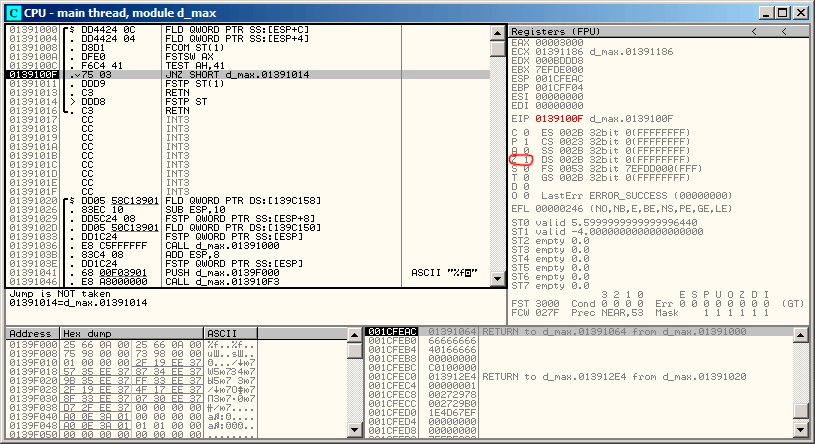
\includegraphics[scale=\FigScale]{patterns/12_FPU/3_comparison/x86/MSVC_Ox/olly2_4.png}
\caption{\olly: \TEST \RU{исполнилась}\EN{executed}}
\label{fig:FPU_comparison_Ox_case2_olly4}
\end{figure}

\begin{figure}[H]
\centering
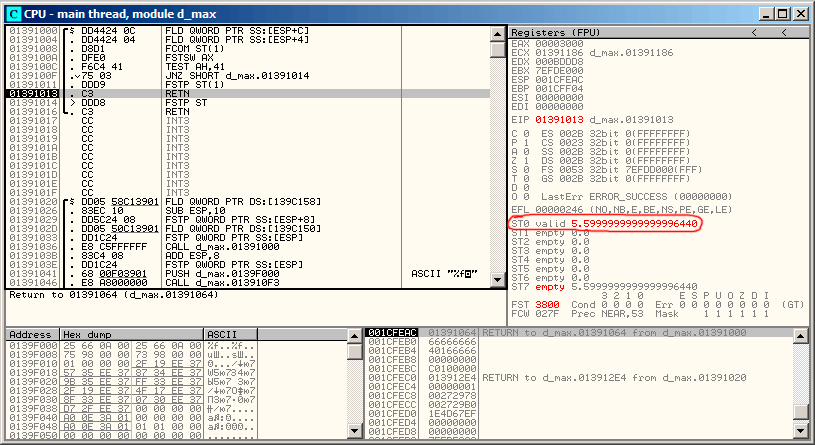
\includegraphics[scale=\FigScale]{patterns/12_FPU/3_comparison/x86/MSVC_Ox/olly2_5.png}
\caption{\olly: \FSTP \RU{исполнилась}\EN{executed}}
\label{fig:FPU_comparison_Ox_case2_olly5}
\end{figure}

\subsubsection{GCC 4.4.1}

\lstinputlisting[caption=GCC 4.4.1]{patterns/12_FPU/3_comparison/x86/GCC_\LANG.asm}

\index{x86!\Instructions!FUCOMPP}
\RU{\FUCOMPP ~--- это почти то же что и \FCOM, только выкидывает из стека оба значения после сравнения, 
а также несколько иначе реагирует на ``не-числа''.}
\EN{\FUCOMPP{}~---is almost like \FCOM, but popping both values from stack and handling 
``not-a-numbers'' differently.}

\index{\RU{Не-числа}\EN{Non-a-numbers} (NaNs)}
\RU{Немного о \IT{не-числах}}\EN{More about \IT{not-a-numbers}}:

\newcommand{\NANFN}{\RU{\footnote{\url{http://ru.wikipedia.org/wiki/NaN}}}
\EN{\footnote{\url{http://en.wikipedia.org/wiki/NaN}}}}

\RU{FPU умеет работать со специальными переменными, которые числами не являются и называются ``не числа'' или 
\gls{NaN}\NANFN{}. 
Это бесконечность, результат деления на ноль, и так далее. Нечисла бывают ``тихие'' и ``сигнализирующие''. 
С первыми можно продолжать работать и далее, а вот если вы попытаетесь совершить какую-то операцию 
с сигнализирующим нечислом, то сработает исключение.}
\EN{FPU is able to deal with a special values which are \IT{not-a-numbers} or 
\gls{NaN}s\NANFN{}. 
These are infinity, result of dividing by $0$, etc. 
Not-a-numbers can be ``quiet'' and ``signaling''. It is possible to continue to work with ``quiet'' NaNs, 
but if one try to do any operation with ``signaling'' NaNs~---an exception will be raised.}

\index{x86!\Instructions!FCOM}
\index{x86!\Instructions!FUCOM}
\RU{Так вот, \FCOM вызовет исключение если любой из операндов ~--- какое-либо нечисло.
\FUCOM же вызовет исключение только если один из операндов именно ``сигнализирующее нечисло''.}
\EN{\FCOM will raise exception if any operand~---\gls{NaN}. 
\FUCOM will raise exception only if any operand~---signaling \gls{NaN} (SNaN).}

\index{x86!\Instructions!SAHF}
\label{SAHF}
\RU{Далее мы видим \SAHF ~--- это довольно редкая инструкция в коде не использующим FPU. 
8 бит из \AH перекладываются в младшие 8 бит регистра статуса процессора в таком порядке: 
\TT{SF:ZF:-:AF:-:PF:-:CF <- AH}.}
\EN{The following instruction is \SAHF~---this is rare instruction in the code which is not use FPU. 
8 bits from AH is movinto into lower 8 bits of CPU flags in the following order: 
\TT{SF:ZF:-:AF:-:PF:-:CF <- AH}.}

\index{x86!\Instructions!FNSTSW}
\RU{Вспомним, что \FNSTSW перегружает интересующие нас биты \CThreeBits в \AH, 
и соответственно они будут в позициях 6, 2, 0 в регистре \AH.}
\EN{Let's remember the \FNSTSW is moving interesting for us bits \CThreeBits into the \AH 
and they will be in positions 6, 2, 0 in the \AH register.}

\RU{Иными словами, пара инструкций \TT{fnstsw  ax / sahf} перекладывает биты \CThreeBits в флаги \ZF, \PF, \CF.}
\EN{In other words, \TT{fnstsw  ax / sahf} instruction pair is moving \CThreeBits into \ZF, \PF, \CF CPU flags.}

\RU{Теперь снова вспомним, какие значения бит \CThreeBits будут при каких результатах сравнения:}
\EN{Now let's also recall, what values of the \CThreeBits bits will be set:}

\begin{itemize}
\item
\RU{Если a больше b в нашем случае, то биты \CThreeBits должны быть выставлены так:}
\EN{If a is greater than b in our example, then \CThreeBits bits will be set as:} 0, 0, 0.
\item
\RU{Если a меньше b, то биты будут выставлены:}\EN{if a is less than b, then bits will be set as:} 0, 0, 1.
\item
\RU{Если a=b, то биты будут выставлены так:}\EN{If a=b, then bits will be set:} 1, 0, 0.
\end{itemize}
% TODO: table?

\RU{Иными словами, после инструкций \FUCOMPP/\FNSTSW/\SAHF, мы получим такое состояние флагов:}
\EN{In other words, after \FUCOMPP/\FNSTSW/\SAHF instructions, we will have these CPU flags states:}

\begin{itemize}
\item
\RU{Если a>b в нашем случае, то флаги будут выставлены так:}
\EN{If a>b, CPU flags will be set as:} \TT{ZF=0, PF=0, CF=0}.
\item
\RU{Если a<b, то флаги будут выставлены:}\EN{If a<b, then CPU flags will be set as:} \TT{ZF=0, PF=0, CF=1}.
\item
\RU{Если a=b, то флаги будут выставлены так:}\EN{If a=b, then CPU flags will be set as:} \TT{ZF=1, PF=0, CF=0}.
\end{itemize}
% TODO: table?

\index{x86!\Instructions!SETNBE}
\index{x86!\Instructions!SETcc}
\index{x86!\Instructions!JNBE}
\RU{Инструкция \SETNBE выставит в \AL единицу или ноль, в зависимости от флагов и условий. 
Это почти аналог \JNBE, за тем лишь исключением, что \SETcc
\footnote{\IT{cc} это \IT{condition code}}
выставляет 1 или 0 в \AL, а \Jcc делает переход или нет. 
\SETNBE запишет 1 если только \TT{CF=0} и \TT{ZF=0}. Если это не так, то запишет $0$ в \AL.}
\EN{How \SETNBE instruction will store 1 or 0 to AL: it is depends of CPU flags. 
It is almost \JNBE instruction counterpart, with the exception the \SETcc 
\footnote{\IT{cc} is \IT{condition code}} is storing 1 or 0 to the \AL, but \Jcc do actual jump or not. 
\SETNBE store 1 only if \TT{CF=0} and \TT{ZF=0}. If it is not true, $0$ will be stored into \AL.}

\RU{\CF будет 0 и \ZF будет 0 одновременно только в одном случае: если a>b.}
\EN{Both \CF is 0 and \ZF is 0 simultaneously only in one case: if a>b.}

\RU{Тогда в \AL будет записана единица, последующий условный переход \JZ взят не будет, 
и функция вернет \TT{\_a}. 
В остальных случаях, функция вернет \TT{\_b}.}
\EN{Then one will be stored to the \AL and the following \JZ will not be triggered and function will 
return {\_a}. In all other cases, {\_b} will be returned.}


\subsubsection{\Optimizing GCC 4.4.1}

\lstinputlisting[caption=\Optimizing GCC 4.4.1]{patterns/12_FPU/3_comparison/x86/GCC_O3.asm.\LANG}

\index{x86!\Instructions!JA}

\ifdefined\ENGLISH
It is almost the same except that \JA is used after \SAHF. 
Actually, conditional jump instructions that check \q{larger}, \q{lesser} or \q{equal} for unsigned number comparison 
(these are \JA, \JAE, \JB, \JBE, \JE/\JZ, \JNA, \JNAE, \JNB, \JNBE, \JNE/\JNZ) check only flags \CF and \ZF.\\
\\
Let's recall where bits \CThreeBits are located in the \TT{AH} register after the execution of \TT{FSTSW}/\FNSTSW:

\begin{center}
\ifdefined\ebook
\begin{bytefield}[endianness=big,bitwidth=0.06\linewidth]{8}
\else
\begin{bytefield}[endianness=big,bitwidth=0.03\linewidth]{8}
\fi
\bitheader{6,2,1,0} \\
\bitbox{1}{} & 
\bitbox{1}{\TT{C3}} & 
\bitbox{3}{} & 
\bitbox{1}{\TT{C2}} & 
\bitbox{1}{\TT{C1}} & 
\bitbox{1}{\TT{C0}}
\end{bytefield}
\end{center}


Let's also recall, how the bits from \TT{AH} are stored into the CPU flags the execution of \SAHF:

\begin{center}
\begin{bytefield}[endianness=big,bitwidth=0.03\linewidth]{8}
\bitheader{7,6,4,2,0} \\
\bitbox{1}{SF} & 
\bitbox{1}{ZF} & 
\bitbox{1}{} & 
\bitbox{1}{AF} & 
\bitbox{1}{} & 
\bitbox{1}{PF} & 
\bitbox{1}{} & 
\bitbox{1}{CF}
\end{bytefield}
\end{center}


After the comparison, the \Cthree and \Czero bits are moved into \ZF and \CF, so the conditional jumps are able work after. \JA is triggering if both \CF are \ZF zero.

Thereby, the conditional jumps instructions listed here can be used after a \FNSTSW/\SAHF instruction pair.

Apparently, the FPU \CThreeBits status bits were placed there intentionally, to easily map them to base CPU flags without additional permutations?
\fi % ENGLISH

\ifdefined\RUSSIAN
Почти всё что здесь есть, уже описано мною, кроме одного: использование \JA после \SAHF. 
Действительно, инструкции условных переходов \q{больше}, \q{меньше} и \q{равно} для сравнения беззнаковых чисел 
(а это \JA, \JAE, \JB, \JBE, \JE/\JZ, \JNA, \JNAE, \JNB, \JNBE, \JNE/\JNZ) проверяют только флаги \CF и \ZF.\\
\\
Вспомним, как биты \CThreeBits располагаются в регистре \TT{AH} после исполнения \TT{FSTSW}/\FNSTSW:

\begin{center}
\ifdefined\ebook
\begin{bytefield}[endianness=big,bitwidth=0.06\linewidth]{8}
\else
\begin{bytefield}[endianness=big,bitwidth=0.03\linewidth]{8}
\fi
\bitheader{6,2,1,0} \\
\bitbox{1}{} & 
\bitbox{1}{\TT{C3}} & 
\bitbox{3}{} & 
\bitbox{1}{\TT{C2}} & 
\bitbox{1}{\TT{C1}} & 
\bitbox{1}{\TT{C0}}
\end{bytefield}
\end{center}


Вспомним также, как располагаются биты из \TT{AH} во флагах CPU после исполнения \SAHF:

\begin{center}
\begin{bytefield}[endianness=big,bitwidth=0.03\linewidth]{8}
\bitheader{7,6,4,2,0} \\
\bitbox{1}{SF} & 
\bitbox{1}{ZF} & 
\bitbox{1}{} & 
\bitbox{1}{AF} & 
\bitbox{1}{} & 
\bitbox{1}{PF} & 
\bitbox{1}{} & 
\bitbox{1}{CF}
\end{bytefield}
\end{center}


Биты \Cthree и \Czero после сравнения перекладываются в флаги \ZF и \CF так, что перечисленные инструкции переходов могут работать. \JA сработает, если \CF и \ZF обнулены.

Таким образом, перечисленные инструкции условного перехода можно использовать после инструкций \FNSTSW/\SAHF.

Может быть, биты статуса FPU \CThreeBits преднамеренно были размещены таким образом, чтобы переноситься на базовые флаги процессора без перестановок?
\fi % RUSSIAN


\subsubsection{GCC 4.8.1 \RU{с оптимизацией \Othree}\EN{with \Othree optimization turned on}}

\EN{Some new FPU instructions were appeared in P6 Intel family}\RU{В линейке процессоров P6 от Intel 
появились новые FPU-инструкции}\footnote{\EN{Starting at}\RU{Начиная с} Pentium Pro, 
Pentium-II, \RU{итд}\EN{etc}}.
\RU{Это}\EN{These are} \TT{FUCOMI} (\RU{сравнить операнды и выставить флаги основного CPU}\EN{compare 
operands and set flags of main CPU}) \AndENRU 
\TT{FCMOVcc} (\RU{работает как}\EN{works like} \TT{CMOVcc}, \RU{но на регистрах FPU}\EN{but on FPU registers}).
\RU{Очевидно, разработчики GCC решили отказаться от поддержки процессоров до линейки P6 (ранние Pentium, итд)}
\EN{Apparently, GCC maintainers decided to drop support of Intel CPUs before P6 family (early Pentiums, etc)}.

\RU{И похоже, FPU уже давно не отдельная часть процессора в линейке P6, так что флаги основного CPU можно
модифицировать из FPU.}
\EN{It seems, FPU is no longer separate unit in P6 Intel family, so now it is possible to modify/check flags 
of main CPU from FPU.}

\RU{Вот что имеем}\EN{So what we got is}:

\lstinputlisting[caption=\Optimizing GCC 4.8.1]{patterns/12_FPU/3_comparison/x86/GCC481_O3.s}

\RU{Не совсем понимаю, зачем здесь \TT{FXCH} (поменять местами операнды)}
\EN{I'm not sure why \TT{FXCH} (swap operands) is here}.
\RU{От нее легко избавиться поменяв местами инструкции \FLD либо заменив 
\TT{FCMOVBE} (\IT{below or equal} --- меньше или равно) на 
\TT{FCMOVA} (\IT{above} --- больше).}
\EN{It's possible to get rid of it easily by swapping two first \FLD instructions or by replacing 
\TT{FCMOVBE} (\IT{below or equal}) by \TT{FCMOVA} (\IT{above}).}
\RU{Должно быть, неаккуратность компилятора}\EN{Probably, compiler's inaccuracy}.

\RU{Так что}\EN{So} \TT{FUCOMI} \EN{compares}\RU{сравниванет} \ST{0} ($a$) \AndENRU \ST{1} ($b$) 
\RU{и затем устанавливает флаги основного CPU}\EN{and then sets main CPU flags}.
\TT{FCMOVBE} \RU{проверяет флаги и копирует}\EN{checks flags and copying} \ST{1} 
(\RU{в тот момент там находится $b$}\EN{$b$ here at the moment}) \RU{в}\EN{to} 
\ST{0} (\RU{там $a$}\EN{$a$ here}) \RU{если}\EN{if} $ST0 (a) <= ST1 (b)$.
\RU{В противном случае}\EN{Otherwise} ($a>b$), \RU{она оставляет}\EN{it leaves} $a$ \InENRU \ST{0}.

\RU{Последняя}\EN{The last} \FSTP \RU{оставляет содержимое}\EN{leaves} \ST{0} 
\RU{на вершине стека, выбрасывая содержимое}\EN{on top of stack discarding} \ST{1}\EN{ contents}.

\RU{Попробуем оттрасировать ф-цию в}\EN{Let's trace this function in} GDB:

\lstinputlisting[caption=\Optimizing GCC 4.8.1 and GDB,numbers=left]{patterns/12_FPU/3_comparison/x86/gdb.txt}

\RU{Используя}\EN{Using} ``ni'', \RU{дадим первым двум инструкциям \FLD исполниться.}
\EN{let's execute two first \FLD instructions.}

\RU{Посмотрим регистры FPU}\EN{Let's examine FPU registers} (\LineENRU 33).

\RU{Как я писал раннее, регистры FPU это скорее кольцевой буфер, нежели стек}
\EN{As I wrote before, FPU registers are circular buffer rather than stack} (\ref{FPU_is_rather_circular_buffer}).
\RU{И}\EN{And} GDB \RU{показывает не регистры}\EN{shows not} \TT{STx} \RU{а внутренние регистры FPU}
\EN{registers, but internal FPU registers} (\TT{Rx}). 
\RU{Стрелка}\EN{Arrow} (\RU{на строке}\EN{at line} 35) 
\RU{указывает на текущую вершину стека.}
\EN{points to the current stack top.}
\RU{Вы можете также увидеть переменную \TT{TOP} в ``Status Word'' (строка 44), там сейчас 6, так что
вершина стека это сейчас внутренний регистр 6.}
\EN{You may also see \TT{TOP} variable in \IT{Status Word} (line 44) it has 6 now, 
so stack top is now in internal register 6.}

\RU{Значения $a$ и $b$ меняются местами после исполнения \TT{FXCH}}\EN{$a$ and $b$ values are swapped 
after \TT{FXCH} executed} (\LineENRU 54).

\TT{FUCOMI} \RU{исполнилась}\EN{executed} (\LineENRU 83). 
\RU{Посмотрим флаги}\EN{Let's see flags}: \CF \RU{выставлен}\EN{is set} (\LineENRU 95).

\TT{FCMOVBE} \RU{действительно скопировал значение $b$ (см.строку 104).}
\EN{is actually copied value of $b$ (see line 104).}

\FSTP \RU{оставляет одно значение на вершине стека}\EN{leaves one value at the top of stack} (\LineENRU 136). 
\RU{Значение \TT{TOP} теперь 7, так что вершина FPU-стека указывает на внутренний регистр 7}\EN{\TT{TOP} value is 
now 7, so FPU stack top is points to internal register 7}.

% TODO task: rewrite the function without FXCH and test it



\ifdefined\IncludeARM
\subsection{ARM}

\subsubsection{\OptimizingXcodeIV (\ARMMode)}

\lstinputlisting[caption=\OptimizingXcodeIV (\ARMMode)]{patterns/12_FPU/3_comparison/ARM/Xcode_ARM.lst.\LANG}

\index{ARM!\Registers!APSR}
\index{ARM!\Registers!FPSCR}
\RU{Очень простой случай.}\EN{A very simple case.}
\RU{Входные величины помещаются в}\EN{The input values are placed into the} \TT{D17} \AndENRU \TT{D16} 
\RU{и сравниваются при помощи инструкции}\EN{registers and then compared using the} 
\TT{VCMPE}\EN{ instruction}.
\RU{Как и в сопроцессорах x86, сопроцессор в ARM имеет свой собственный регистр статуса и флагов}
\EN{Just like in the x86 coprocessor, the ARM coprocessor has its own status and flags register}, (\ac{FPSCR}),
\RU{потому как есть необходимость хранить специфичные для его работы флаги.}
\EN{since there is a need to store coprocessor-specific flags.}
% TODO -> расписать регистр по битам
\index{ARM!\Instructions!VMRS}
\RU{И так же, как и в x86}\EN{And just like in x86}, 
\RU{в ARM нет инструкций условного перехода}
\EN{there are no conditional jump instruction in ARM}, 
\RU{проверяющих биты в регистре статуса сопроцессора}\EN{that can check bits in the status register of the coprocessor}, 
\RU{так что имеется инструкция}\EN{so there is} \TT{VMRS}
\RU{, копирующая 4 бита}\EN{, which copies 4 bits} (N, Z, C, V) 
\RU{из статуса сопроцессора в биты \IT{общего} статуса (регистр \ac{APSR}).}
\EN{from the coprocessor status word into bits of the \IT{general} status register (\ac{APSR}).}

\index{ARM!\Instructions!VMOVGT}
\TT{VMOVGT} \RU{это аналог}\EN{is the analog of the} \TT{MOVGT}, 
\RU{инструкция для D-регистров, сработающая если при сравнении один операнд был больше чем второй}
\EN{instruction for D-registers, it executes if one operand is greater than the other while comparing} 
(\IT{GT\EMDASH{}Greater Than}). 

\RU{Если она сработает}\EN{If it gets executed}, 
\RU{в \TT{D16} запишется значение $b$}\EN{the value of $b$ will be written into \TT{D16}} 
\RU{, лежащее в тот момент в}\EN{(that is currently stored in in} \TT{D17} \EN{)}.

\RU{В обратном случае}\EN{Otherwise}, 
\RU{в \TT{D16} останется лежать значение $a$.}
\EN{the value of $a$ will stay in the \TT{D16} register.}

\index{ARM!\Instructions!VMOV}
\RU{Предпоследняя инструкция \TT{VMOV} подготовит то что было в \TT{D16} для возврата через 
пару регистров \Reg{0} и \Reg{1}.}
\EN{The penultimate instruction \TT{VMOV} will prepare the value in the \TT{D16} register for returning it via the \Reg{0} and \Reg{1}
register pair.}

\subsubsection{\OptimizingXcodeIV (\ThumbTwoMode)}

\begin{lstlisting}[caption=\OptimizingXcodeIV (\ThumbTwoMode)]
VMOV            D16, R2, R3 ; b
VMOV            D17, R0, R1 ; a
VCMPE.F64       D17, D16
VMRS            APSR_nzcv, FPSCR
IT GT 
VMOVGT.F64      D16, D17
VMOV            R0, R1, D16
BX              LR
\end{lstlisting}

\RU{Почти то же самое что и в предыдущем примере, за парой отличий.}
\EN{Almost the same as in the previous example, however slightly different.}
\RU{Как мы уже знаем, многие инструкции в режиме ARM можно дополнять условием.}
\EN{As we already know, many instructions in ARM mode can be supplemented by condition predicate.}

\RU{Но в режиме thumb такого нет}
\EN{But there is no such thing in thumb mode}. 
\RU{В 16-битных инструкций просто нет места для лишних 4 битов, при помощи
которых можно было бы закодировать условие выполнения.}
\EN{There is no space in the 16-bit instructions for 4 more bits in which conditions can be encoded.}

\index{ARM!\ThumbTwoMode}
\RU{Поэтому в thumb-2 добавили возможность дополнять thumb-инструкции условиями.}
\EN{However, thumb-2 was extended to make it possible to specify predicates to old thumb instructions.}

\RU{Здесь, в листинге, сгенерированном при помощи \IDA, мы видим инструкцию \TT{VMOVGT}, 
такую же как и в предыдущем примере.}
\EN{Here, in the \IDA-generated listing, we see the \TT{VMOVGT} instruction, as in previous example.}

\RU{В реальности}\EN{In fact}, 
\RU{там закодирована обычная инструкция \TT{VMOV}}
\EN{the usual \TT{VMOV} is encoded there}, 
\RU{просто \IDA добавила суффикс \TT{-GT} к ней}
\EN{but \IDA adds the \TT{-GT} suffix to it}, 
\RU{потому что перед этой инструкцией стоит \TT{``IT GT''}}
\EN{since there is a \TT{``IT GT''} instruction placed right before it}.

\label{ARM_Thumb_IT}
\index{ARM!\Instructions!IT}
\index{ARM!if-then block}
\EN{The}\RU{Инструкция} \TT{IT} \RU{определяет так называемый}\EN{instruction defines a so-called} \IT{if-then block}. 
\RU{После этой инструкции, можно указывать до четырех инструкций, к которым будет добавлен суффикс условия.}
\EN{After the instruction it is possible to place up to 4 instructions to which a predicate suffix will be added.}
\RU{В нашем примере}\EN{In our example}, \TT{``IT GT''} \RU{означает,}\EN{implies}
\RU{что следующая за ней инструкция будет исполнена}\EN{that the next instruction will be executed}, 
\RU{если условие}\EN{if the} \IT{GT} (\IT{Greater Than}) \RU{справедливо}\EN{condition is true}.

\index{Angry Birds}
\RU{Теперь более сложный пример, кстати, из}\EN{Here is a more complex code fragment, by the way, from} 
``Angry Birds'' (\RU{для}\EN{for} iOS):

\begin{lstlisting}[caption=Angry Birds Classic]
ITE NE
VMOVNE          R2, R3, D16
VMOVEQ          R2, R3, D17
\end{lstlisting}

\TT{ITE} \RU{означает}\EN{stands for} \IT{if-then-else} 
\RU{и кодирует суффиксы для двух следующих за ней инструкций.}
\EN{and it encodes suffixes for the next two instructions.}
\RU{Первая из них исполнится, если условие, закодированное в}
\EN{The first instruction will execute if the condition encoded in} \TT{ITE} (\IT{NE, not equal}) 
\RU{будет в тот момент справедливо}\EN{is true at},
\RU{а вторая ~--- если это условие не сработает}\EN{and the 
second~---if the condition is not true}.
(\RU{Обратное условие от}\EN{The inverse condition of} \TT{NE} \RU{это}\EN{is} \TT{EQ} (\IT{equal})).

\index{Angry Birds}
\RU{Еще чуть сложнее}\EN{One more that's slightly harder}, 
\RU{и снова этот фрагмент из}\EN{which is also from} ``Angry Birds'':

\begin{lstlisting}[caption=Angry Birds Classic]
ITTTT EQ
MOVEQ           R0, R4
ADDEQ           SP, SP, #0x20
POPEQ.W         {R8,R10}
POPEQ           {R4-R7,PC}
\end{lstlisting}

\RU{4 символа ``T'' в инструкции означают что 4 следующие инструкции будут исполнены если условие соблюдается.}
\EN{4 ``T'' symbols in the instruction mnemonic mean 
that the 4 instructions that follow will be executed if the condition is true.}
\RU{Поэтому \IDA добавила ко всем четырем инструкциям суффикс}
\EN{That's why \IDA adds the} \TT{-EQ}\EN{ suffix
to each one of them}. 

\RU{А если бы здесь было, например,}\EN{And if there was be, for example,}
\TT{ITEEE EQ} (\IT{if-then-else-else-else}), 
\RU{тогда суффиксы для следующих четырех инструкций были бы расставлены так:}
\EN{then the suffixes would have been set as follows:}

\begin{lstlisting}
-EQ
-NE
-NE
-NE
\end{lstlisting}

\index{Angry Birds}
\RU{Еще фрагмент из}\EN{Another fragment from} ``Angry Birds'':

\begin{lstlisting}[caption=Angry Birds Classic]
CMP.W           R0, #0xFFFFFFFF
ITTE LE
SUBLE.W         R10, R0, #1
NEGLE           R0, R0
MOVGT           R10, R0
\end{lstlisting}

\TT{ITTE} (\IT{if-then-then-else}) \RU{означает что первая и вторая инструкции исполнятся}
\EN{implies that the 1st and 2nd instructions will be executed }
\RU{, если условие}\EN{if the} \TT{LE} (\IT{Less or Equal}) \RU{справедливо}\EN{condition is true},
\RU{а третья}\EN{and the 3rd}\EMDASH\RU{если справедливо обратное условие}\EN{if the inverse condition} 
(\TT{GT}\EMDASH\IT{Greater Than})\EN{ is true}.

\RU{Компиляторы способны генерировать далеко не все варианты.}
\EN{Compilers usually don't generate all possible combinations.}
\index{Angry Birds}
\RU{Например, в вышеупомянутой игре ``Angry Birds'' (версия \IT{classic} для iOS)}
\EN{For example, in the mentioned ``Angry Birds'' game (\IT{classic} version for iOS)}
\RU{встречаются только такие варианты инструкции \TT{IT}}\EN{only these variants of the \TT{IT} instruction are used}: 
\TT{IT}, \TT{ITE}, \TT{ITT}, \TT{ITTE}, \TT{ITTT}, \TT{ITTTT}.
\index{\GrepUsage}
\RU{Как я это узнал?}\EN{How did I learn this?}
\RU{В \IDA можно сгенерировать листинг, так я и сделал, только в опциях я установил так 
чтобы показывались 4 байта для каждого опкода.}
\EN{In \IDA It is possible to produce listing files, so I created them with an option 
to show 4 bytes for each opcode .}
\RU{Затем, зная, что старшая часть 16-битного опкода (\TT{IT} это \TT{0xBF}), я сделал при помощи \TT{grep} это:}
\EN{Then, knowing the high part of the 16-bit opcode (\TT{IT} is \TT{0xBF}),
I did the following using \TT{grep}:}

\begin{lstlisting}
cat AngryBirdsClassic.lst | grep " BF" | grep "IT" > results.lst
\end{lstlisting}

\index{ARM!\ThumbTwoMode}
\RU{Кстати, если писать на ассемблере для режима thumb-2 вручную, и дополнять инструкции суффиксами
условия, то ассемблер автоматически будет добавлять инструкцию \TT{IT} с соответствующими флагами, там,
где надо.}
\EN{By the way, if you program in ARM assembly language manually for thumb-2 mode, 
and you add conditional suffixes,
the assembler will add the \TT{IT} instructions automatically with the required flags where it is necessary.}

\subsubsection{\NonOptimizingXcodeIV (\ARMMode)}

\begin{lstlisting}[caption=\NonOptimizingXcodeIV (\ARMMode)]
b               = -0x20
a               = -0x18
val_to_return   = -0x10
saved_R7        = -4

                STR             R7, [SP,#saved_R7]!
                MOV             R7, SP
                SUB             SP, SP, #0x1C
                BIC             SP, SP, #7
                VMOV            D16, R2, R3
                VMOV            D17, R0, R1
                VSTR            D17, [SP,#0x20+a]
                VSTR            D16, [SP,#0x20+b]
                VLDR            D16, [SP,#0x20+a]
                VLDR            D17, [SP,#0x20+b]
                VCMPE.F64       D16, D17
                VMRS            APSR_nzcv, FPSCR
                BLE             loc_2E08
                VLDR            D16, [SP,#0x20+a]
                VSTR            D16, [SP,#0x20+val_to_return]
                B               loc_2E10

loc_2E08
                VLDR            D16, [SP,#0x20+b]
                VSTR            D16, [SP,#0x20+val_to_return]

loc_2E10
                VLDR            D16, [SP,#0x20+val_to_return]
                VMOV            R0, R1, D16
                MOV             SP, R7
                LDR             R7, [SP+0x20+b],#4
                BX              LR
\end{lstlisting}

\RU{Почти то же самое что мы уже видели}\EN{Almost the same as we already saw}, 
\RU{но много избыточного кода из-за хранения $a$ и $b$, 
а также выходного значения, в локальном стеке.}
\EN{but there is too much redundant code because the $a$ and $b$ variables are stored in the local stack, as well
as the return value.}

\subsubsection{\OptimizingKeilVI (\ThumbMode)}

\begin{lstlisting}[caption=\OptimizingKeilVI (\ThumbMode)]
                PUSH    {R3-R7,LR}
                MOVS    R4, R2
                MOVS    R5, R3
                MOVS    R6, R0
                MOVS    R7, R1
                BL      __aeabi_cdrcmple
                BCS     loc_1C0
                MOVS    R0, R6
                MOVS    R1, R7
                POP     {R3-R7,PC}

loc_1C0
                MOVS    R0, R4
                MOVS    R1, R5
                POP     {R3-R7,PC}
\end{lstlisting}

\RU{Keil не генерирует FPU-инструкции, потому что не 
рассчитывает на то что они будет поддерживаться, а простым сравнением побитово здесь не обойтись.}
\EN{Keil doesn't generate FPU-instructions since it cannot rely on them being
supported on the target CPU, and it cannot be done by straightforward bitwise comparing.}
%TODO: why?
\RU{Для сравнения вызывается библиотечная функция}\EN{So it calls an external library
function to do the comparison:} \TT{\_\_aeabi\_cdrcmple}. 
\index{ARM!\Instructions!BCS}\\
\\
N.B. \RU{Результат
сравнения эта функция оставляет в флагах, чтобы следующая за вызовом инструкция}
\EN{The result of the comparison is to be left in the flags by this function, so the following}
\TT{BCS} (\IT{Carry set - Greater than or equal})
\RU{могла работать без дополнительного кода.}\EN{instruction can work without any additional code.}

 

\subsection{ARM64}

\subsubsection{\Optimizing GCC (Linaro) 4.9}

\lstinputlisting{patterns/12_FPU/3_comparison/ARM/ARM64_GCC_O3.lst.\LANG}

\EN{The}\RU{В} ARM64 \ac{ISA} \RU{теперь есть FPU-инструкции, устанавливающие флаги CPU}\EN{has FPU-instructions 
which set} \ac{APSR} \RU{вместо}\EN{the CPU flags instead of} \ac{FPSCR} \EN{for convenience}\RU{для удобства}.
\EN{The}\ac{FPU} \RU{больше не отдельное устройство (по крайней мере логически)}\EN{is not a separate device here 
anymore (at least, logically)}.
\myindex{ARM!\Instructions!FCMPE}
\RU{Это}\EN{Here we see} \INS{FCMPE}. \RU{Она сравнивает два значения, переданных в}\EN{It compares the two values 
passed in} \RegD{0} \AndENRU \RegD{1} 
(\RU{а это первый и второй аргументы функции}\EN{which are the first and second arguments of the function})
\RU{и выставляет флаги в}\EN{and sets} \ac{APSR}\EN{ flags} (N, Z, C, V).

\myindex{ARM!\Instructions!FCSEL}
\INS{FCSEL} (\IT{Floating Conditional Select}) \RU{копирует значение}\EN{copies the value of} \RegD{0} \OrENRU 
\RegD{1} \RU{в}\EN{into} \RegD{0} \RU{в зависимости от условия}\EN{depending on the condition} 
(\GTT{GT}\EMDASH{}Greater Than\RU{\EMDASH{}больше чем}),
\RU{и снова, она использует флаги в регистре}\EN{and again, it uses flags in} \ac{APSR} \RU{вместо}\EN{register
instead of} \ac{FPSCR}.
\RU{Это куда удобнее, если сравнивать с тем набором инструкций, что был в процессорах раньше.}
\EN{This is much more convenient, compared to the instruction set in older CPUs.}

\RU{Если условие верно}\EN{If the condition is true} (\GTT{GT}), \RU{тогда значение из}\EN{then the value of} \RegD{0} 
\RU{копируется в}\EN{is copied into} \RegD{0} (\RU{т.е. ничего не происходит}\EN{i.e., nothing happens}).
\RU{Если условие не верно, то значение}\EN{If the condition is not true, the value of} \RegD{1} 
\RU{копируется в}\EN{is copied into} \RegD{0}.

\subsubsection{\NonOptimizing GCC (Linaro) 4.9}

\lstinputlisting{patterns/12_FPU/3_comparison/ARM/ARM64_GCC.lst.\LANG}

\RU{Неоптимизирующий GCC более многословен}\EN{Non-optimizing GCC is more verbose}.
\RU{В начале функция сохраняет значения входных аргументов в локальном стеке}
\EN{First, the function saves its input argument values in the local stack} (\IT{Register Save Area}).
\RU{Затем код перезагружает значения в регистры}\EN{Then the code reloads these values into registers}
\RegX{0}/\RegX{1} \RU{и наконец копирует их в}\EN{and finally copies them to} 
\RegD{0}/\RegD{1} \RU{для сравнения инструкцией}\EN{to be compared using} \INS{FCMPE}. 
\RU{Много избыточного кода, но так работают неоптимизирующие компиляторы}\EN{A lot of redundant code, 
but that is how non-optimizing compilers work}.
\INS{FCMPE} \RU{сравнивает значения и устанавливает флаги в}\EN{compares the values and sets the} \ac{APSR}\EN{ flags}.
\RU{В этот момент компилятор ещё не думает о более удобной инструкции}\EN{At this moment, 
the compiler is not thinking yet about the more convenient} \INS{FCSEL}\RU{, так что он работает старым 
методом}\EN{ instruction, so it proceed using old methods}: 
\RU{использует инструкцию}\EN{using the} \INS{BLE}\EN{ instruction} (\IT{Branch if Less than or Equal}\RU{ (переход
если меньше или равно)}).
\RU{В одном случае}\EN{In the first case} ($a>b$)\EN{, the value of}\RU{ значение} $a$ \RU{перезагружается в}\EN{gets loaded 
into} \RegX{0}.
\RU{В другом случае}\EN{In the other case} ($a<=b$)\EN{, the value of}\RU{ значение} $b$ \RU{загружается в}\EN{gets loaded into} 
\RegX{0}.
\RU{Наконец, значение из}\EN{Finally, the value from} \RegX{0} \RU{копируется в}\EN{gets copied into} \RegD{0}, 
\RU{потому что возвращаемое значение оставляется в этом регистре}\EN{because the return value needs to be in this 
register}.

\myparagraph{\Exercise}

\RU{Для упражнения вы можете попробовать оптимизировать этот фрагмент кода вручную, удалив избыточные инструкции,
но не добавляя новых (включая \INS{FCSEL})}\EN{As an exercise, you can try optimizing this piece of code 
manually by removing redundant instructions and not introducing new ones (including \INS{FCSEL})}.

\subsubsection{\Optimizing GCC (Linaro) 4.9\EMDASH{}float}

\RU{Перепишем пример. Теперь здесь \Tfloat вместо \Tdouble.}%
\EN{Let's also rewrite this example to use \Tfloat instead of \Tdouble.}

\begin{lstlisting}
float f_max (float a, float b)
{
	if (a>b)
		return a;

	return b;
};
\end{lstlisting}

\lstinputlisting{patterns/12_FPU/3_comparison/ARM/ARM64_GCC_O3_float.lst.\LANG}

\RU{Всё то же самое, только используются S-регистры вместо D-.}
\EN{It is the same code, but the S-registers are used instead of D- ones.}
\RU{Так что числа типа \Tfloat передаются в 32-битных S-регистрах (а это младшие части 64-битных D-регистров).}
\EN{It's because numbers of type \Tfloat are passed in 32-bit S-registers (which are in fact the lower parts of the 64-bit D-registers).}


\fi
\ifdefined\IncludeMIPS
\subsection{MIPS}

\index{MIPS!\Registers!FCCR}
\EN{The co-processor of the MIPS processor has a condition bit which can be set in the FPU and checked in the CPU.}
\RU{В сопроцессоре MIPS есть бит результата, который устанавливается в FPU и проверяется в CPU.}
\EN{Earlier MIPS-es have only one condition bit (called FCC0), later ones have 8 (called FCC7-FCC0).}
\RU{Ранние MIPS имели только один бит (с названием FCC0), а у поздних их 8 (с названием FCC7-FCC0).}
\RU{Этот бит (или биты) находятся в регистре с названием FCCR.}
\EN{This bit (or bits) are located in the register called FCCR.}

\lstinputlisting[caption=\Optimizing GCC 4.4.5 (IDA)]{patterns/12_FPU/3_comparison/MIPS_O3_IDA.lst.\LANG}

\index{MIPS!\Instructions!C.LT.D}
\TT{C.LT.D} \EN{compares two values}\RU{сравнивает два значения}. 
\TT{LT} \EN{is the condition}\RU{это условие} \q{Less Than}\RU{ (меньше чем)}.
\TT{D} \EN{implies values of type}\RU{означает переменные типа} \Tdouble.
\EN{Depending on the result of the comparison, the FCC0 condition bit is either set or cleared.}
\RU{В зависимости от результата сравнения, бит FCC0 устанавливается или очищается.}

\index{MIPS!\Instructions!BC1T}
\index{MIPS!\Instructions!BC1F}
\TT{BC1T} \EN{checks the FCC0 bit and jumps if the bit is set}\RU{проверяет бит FCC0 и делает переход, если бит выставлен}.
\TT{T} \EN{mean that the jump is to be taken if the bit is set}\RU{означает что переход произойдет если бит выставлен} (\q{True}).
\EN{There is also the instruction}\RU{Имеется также инструкция} \q{BC1F} \EN{which jumps if the bit is cleared}\RU{которая сработает, если бит сброшен} (\q{False}).

\RU{В зависимости от перехода один из аргументов функции помещается в регистр \$F0.}
\EN{Depending on the jump, one of function arguments is placed into \$F0.}

\fi
